\documentclass[12pt]{beamer}
%\documentclass[20pt,handout]{beamer}
\usetheme{Darmstadt}
\usepackage{graphicx}
%\usepackage[german]{babel}
\usepackage{ngerman}
\usepackage[T1]{fontenc}
\usepackage[utf8]{inputenc}
\usepackage{tikz}
\setbeamertemplate{footline}[frame number]

\newcommand{\cc}[1]{\includegraphics[height=4mm]{img/#1.png}\hspace{1mm}}
\usepackage{ifthen}
\newcommand{\license}[2][]{\\#2\ifthenelse{\equal{#1}{}}{}{\\\scriptsize\url{#1}}}
\usepackage{textcomp}
\usepackage{hyperref}

\pgfdeclareimage[height=.6cm]{c3d2logo}{./img/c3d2.pdf}


\pgfdeclarelayer{foreground}
\pgfsetlayers{main,foreground}
\logo{\pgfputat{\pgfxy(-1,0)}{\pgfbox[center,base]{\pgfuseimage{c3d2logo}}}}


\title{Wie schütze ich mich vor Überwachung?}
\author{\small Stephan Thamm und Stefan B"ocker\\\large Chaos Computer Club Dresden}
\date{14.10.2014}

\begin{document}
\maketitle

\section{Einleitung}
\subsection{}

\begin{frame}
  \frametitle{Chaos Computer Club}
  \begin{figure}
    
\includegraphics[height=0.7\textheight]{img/fingerabdruck.jpg}
  \end{figure}
\end{frame}

\begin{frame}
  \frametitle{Chaos Computer Club}
  \begin{figure}
    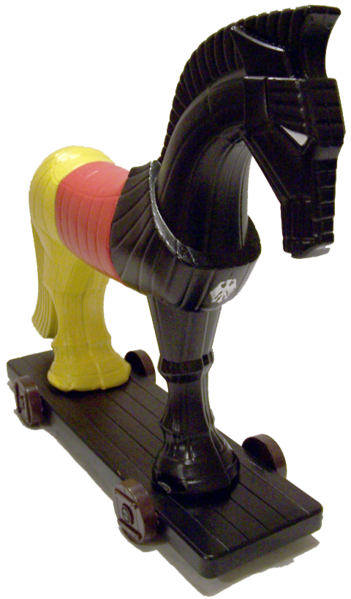
\includegraphics[height=0.7\textheight]{img/trojaner.png}
  \end{figure}
\end{frame}

\begin{frame}
    \frametitle{Chaos Computer Club}
    \begin{itemize}
      \item<1-> Chaos Computer Club Dresden (\url{http://c3d2.de})          
      \item<2-> Datenspuren: September 2015 (\url{http://datenspuren.de})
      \item<3-> Podcasts (\url{http://pentamedia.de})
      \item<4-> Chaos macht Schule
    \end{itemize}
\end{frame}

\begin{frame}
    \frametitle{Bundespräsident Gauck zur NSA-Überwachung}
    \begin{center}
      ``Wir wissen z.B., dass es nicht so ist, wie bei der Stasi und dem KGB, dass es dicke Aktenbände gibt, wo unsere Gesprächsinhalte alle aufgeschrieben und schön abgeheftet sind. Das ist es nicht.''
      (Gauck, 30.06.2013 im ZDF-Sommerinterview)
    \end{center}
\end{frame}

\section{Datensammler}
\subsection{}
\begin{frame}
    \frametitle{Stasi vs. NSA}
    \begin{center}
	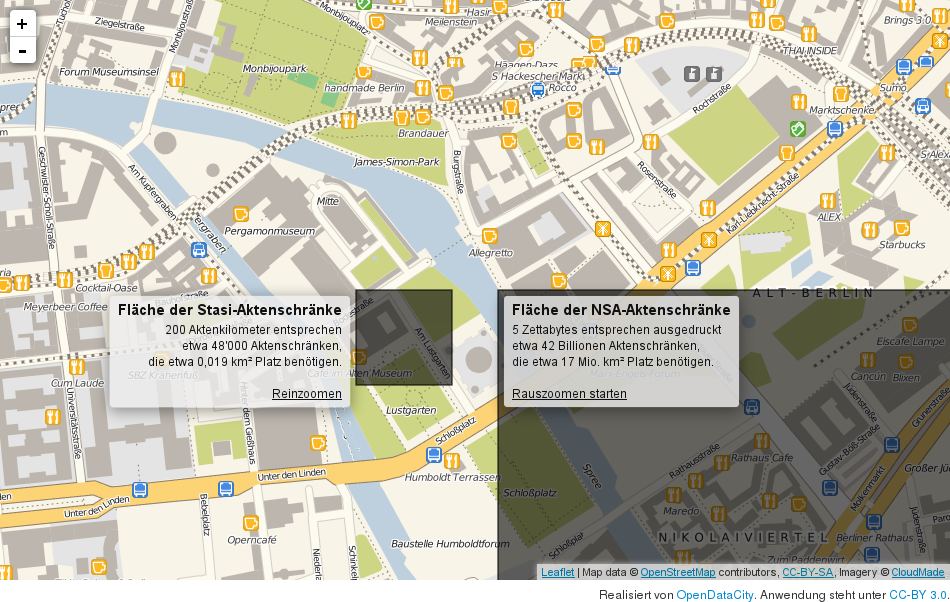
\includegraphics[height=0.7\textheight]{img/akten1.png}
    \end{center}
\end{frame}

\begin{frame}
    \frametitle{Stasi vs. NSA}
    \begin{center}
	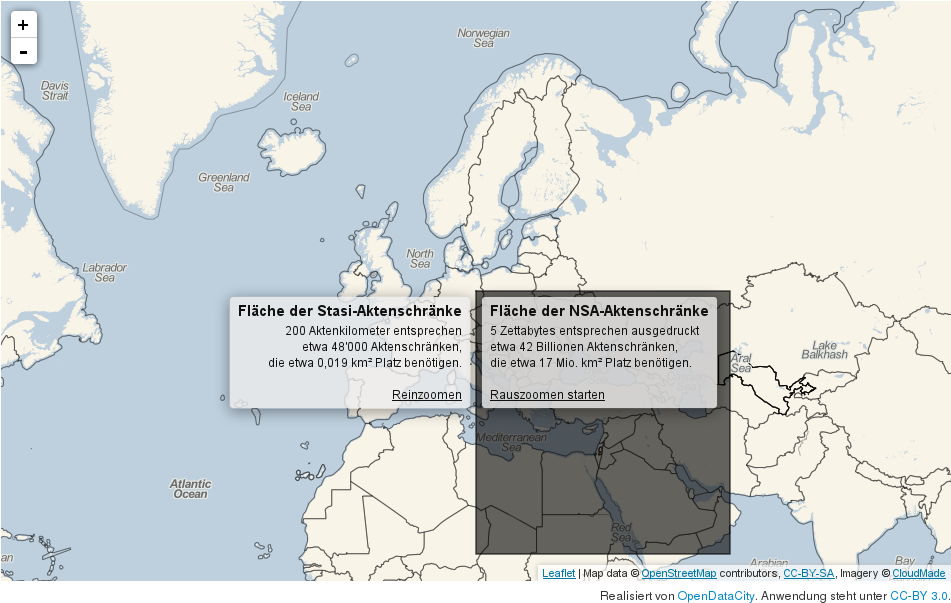
\includegraphics[height=0.7\textheight]{img/akten2.png}
    \end{center}
\end{frame}

\begin{frame}
    \frametitle{NSA-Skandal}
    \begin{center}
	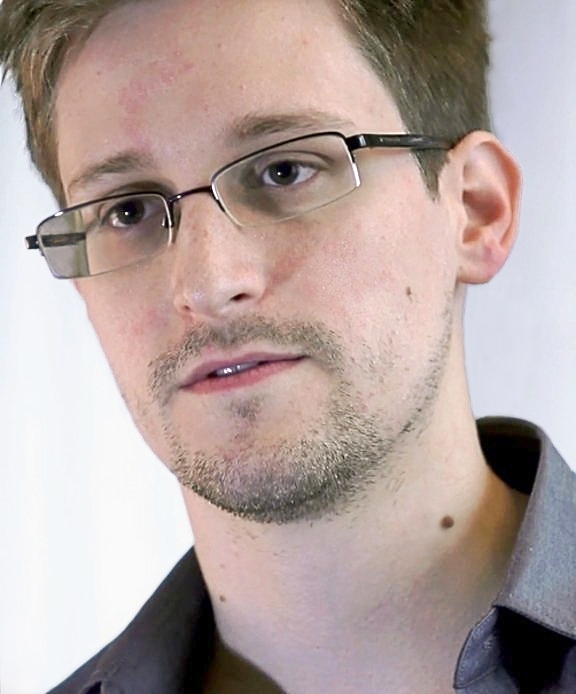
\includegraphics[height=0.7\textheight]{img/snowden.jpg}
	\\{\small \href{https://commons.wikimedia.org/wiki/File:Edward_Snowden.jpg\#mediaviewer/File:Edward_Snowden-2.jpg}{Grafik}: \href{https://creativecommons.org/licenses/by/3.0/}{\cc{by}} Laura Poitras / Praxis Films}
    \end{center}	
\end{frame}

\begin{frame}
    \frametitle{Prism}
    \begin{center}
	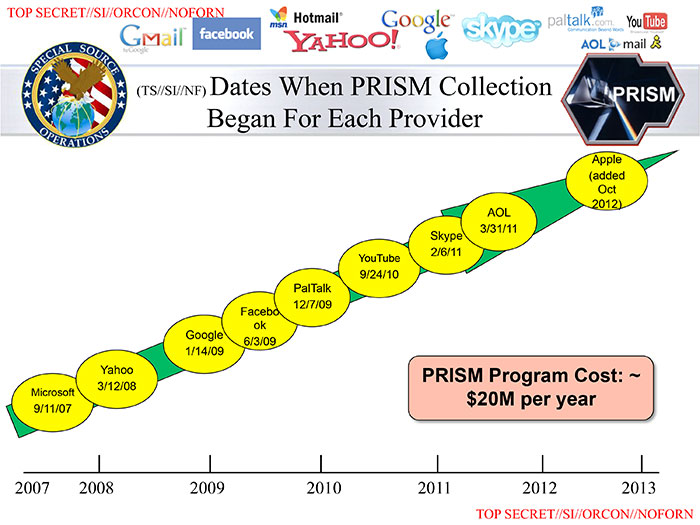
\includegraphics[height=0.7\textheight]{img/prism.jpg}
    \end{center}
\end{frame}

\begin{frame}
  \frametitle{Stasi vs. NSA}
    \begin{center}
      
\includegraphics[height=5cm]{img/prism_netzpolitik.png}
    \end{center}
\end{frame}

\begin{frame}
  \frametitle{Vorratsdatenspeicherung (USA)}
    \begin{center}
      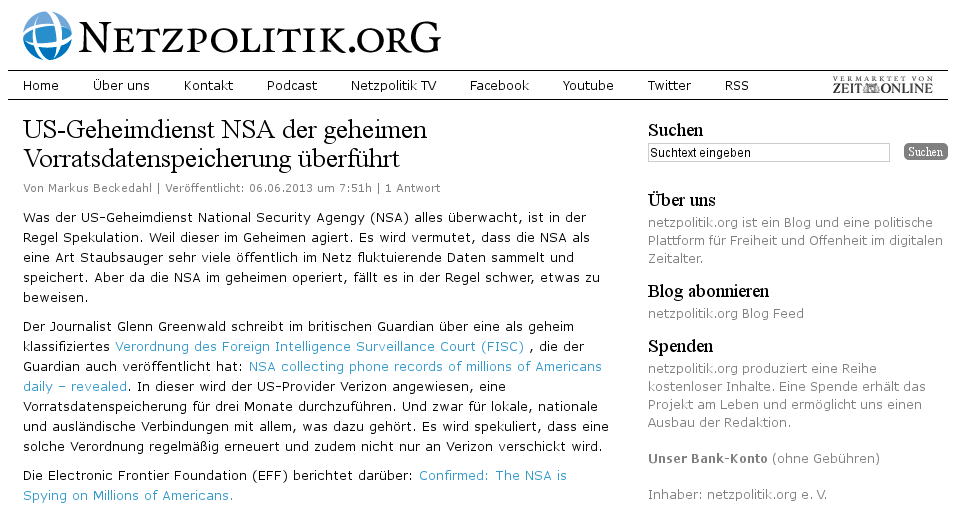
\includegraphics[height=5cm]{img/netzpolitik-verizon.png}
    \end{center}
\end{frame}

\begin{frame}
  \frametitle{Vorratsdatenspeicherung (Deutschland)}
    \begin{center}
      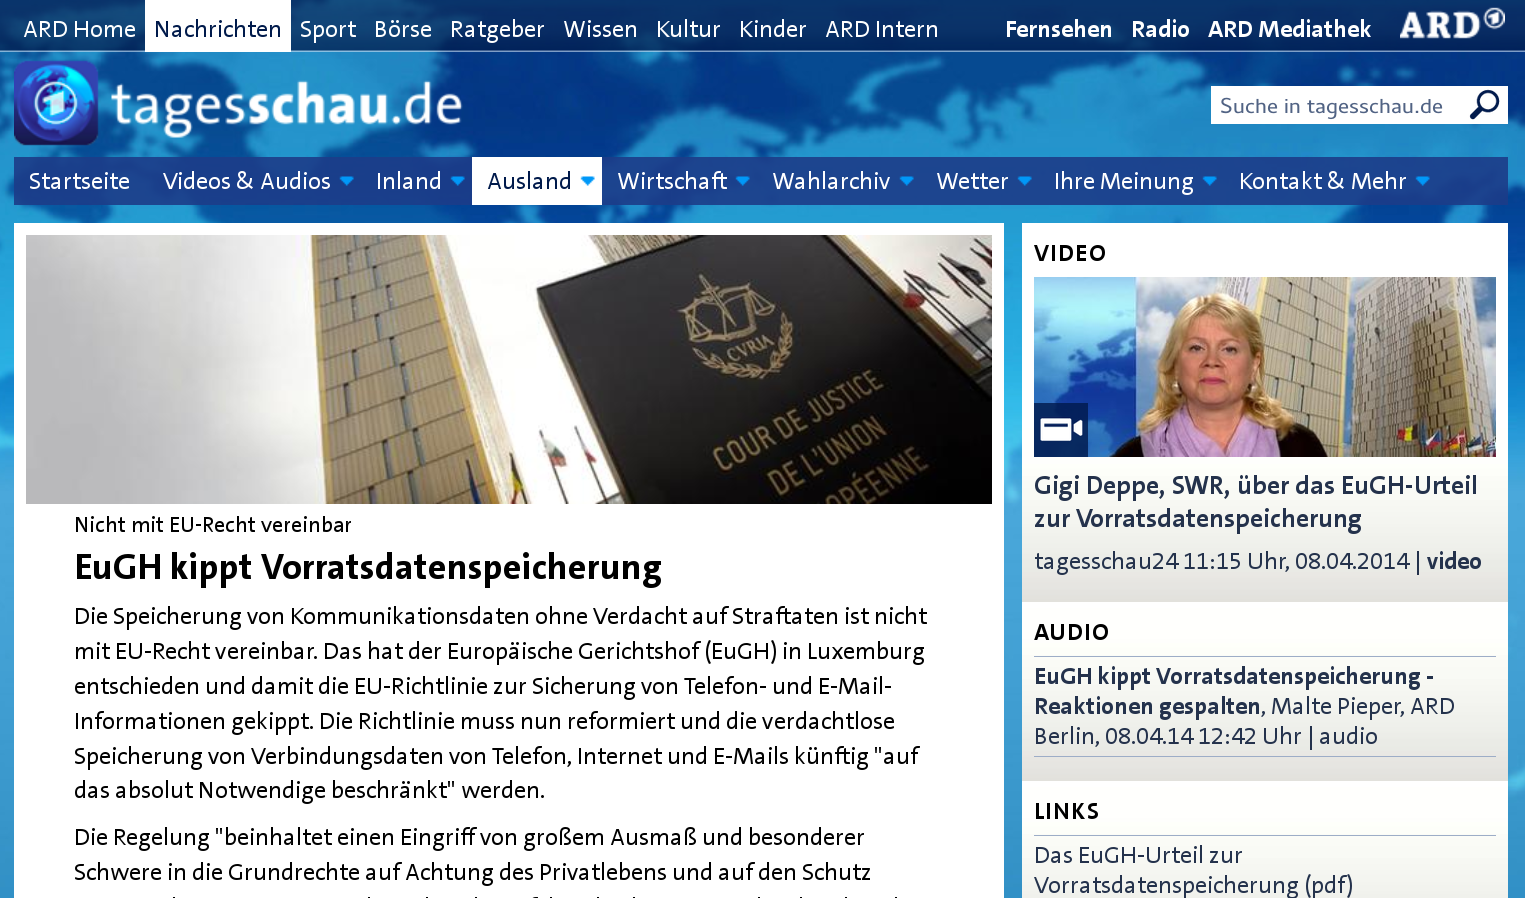
\includegraphics[height=5cm]{img/tagesschau-vds.png}
    \end{center}
\end{frame}

\begin{frame}
  \frametitle{Metadaten}
  \begin{itemize}
    \item Handynetz
      \begin{itemize}
        \item Telefonnummern
        \item Zeitpunkt und Dauer (Telefonate, SMS)
        \item Funkzelle (Ort)
      \end{itemize}
    \item Internet
      \begin{itemize}
        \item IP-Adresse
        \item Alle Verbindungen
        \item Email: Adressen von Sender und Empfänger, Zugriff
      \end{itemize}
  \end{itemize}
\end{frame}

\begin{frame}
    \frametitle{Metadaten}
    \begin{center}
	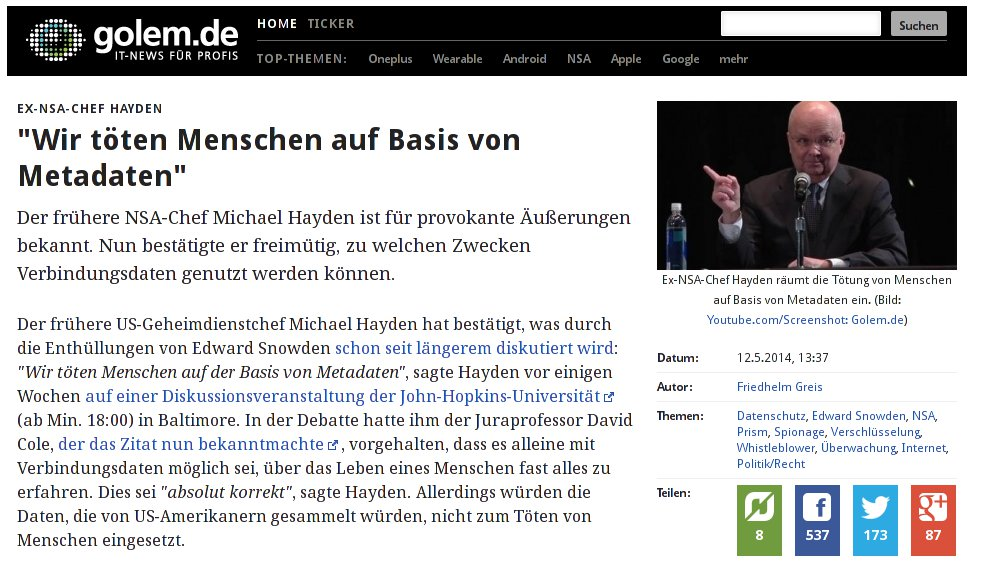
\includegraphics[height=0.7\textheight]{img/wekillpeople.jpg}
    \end{center}
\end{frame}

\section{Technische Gegenmaßnahmen}
\subsection{}
\begin{frame}
    \frametitle{Verschlüsselung allgemein}
    \begin{center}
	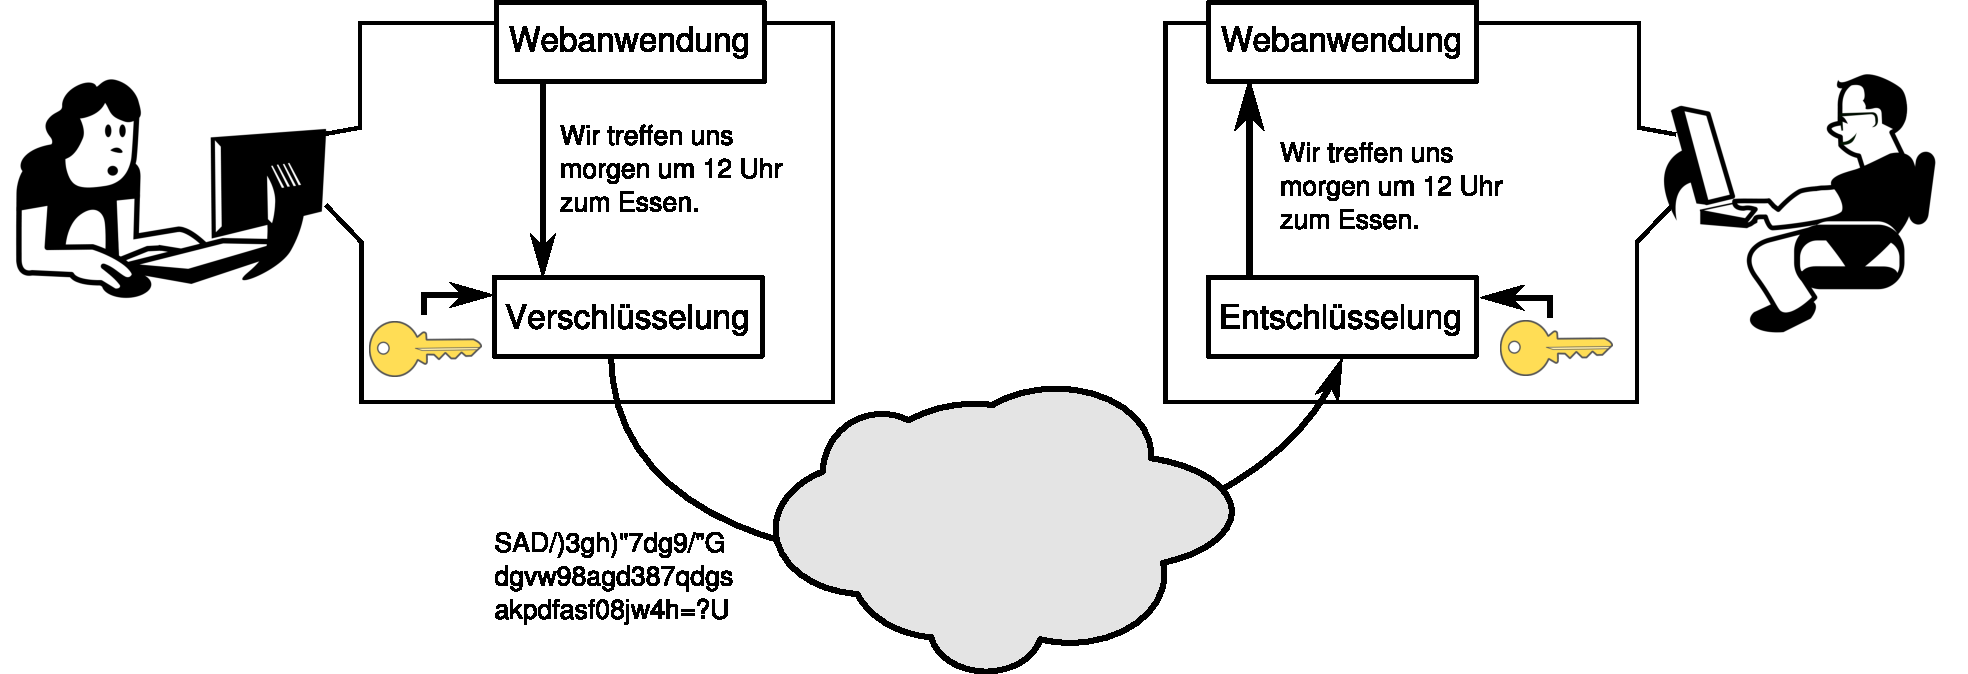
\includegraphics[width=\textwidth]{img/krypto.pdf}
    \end{center}	
\end{frame}

\begin{frame}
    \frametitle{Symmetrische Verschlüsselung}
    \begin{center}
	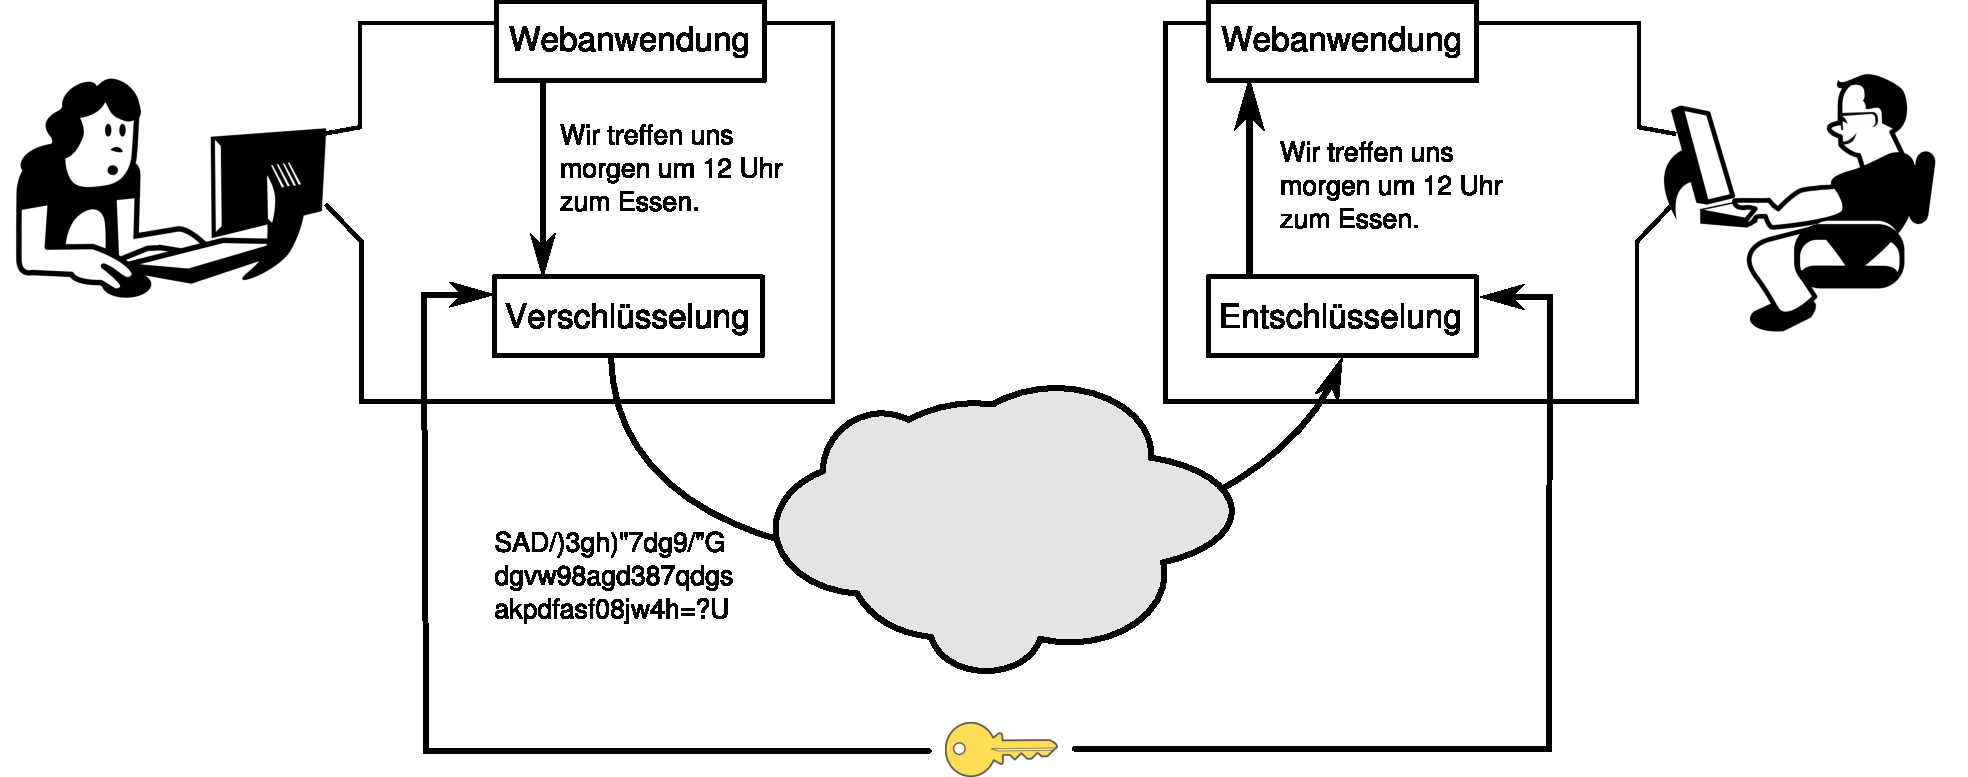
\includegraphics[width=\textwidth]{img/krypto_symmetric.pdf}
    \end{center}	
\end{frame}

\begin{frame}
    \frametitle{Asymmetrische Verschlüsselung}
    \begin{center}
	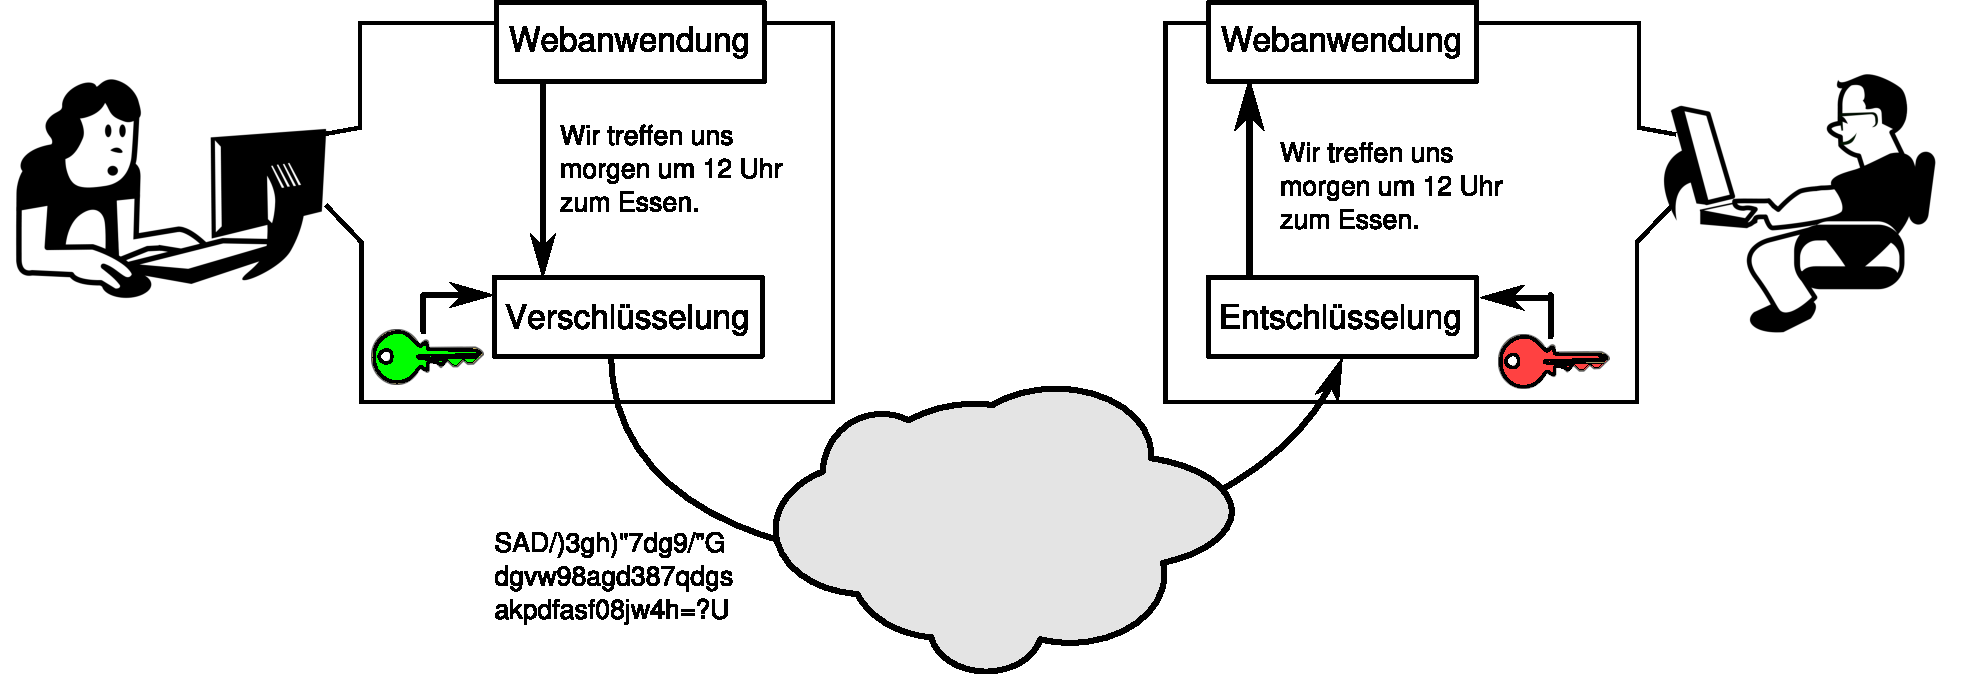
\includegraphics[width=\textwidth]{img/krypto_asymmetric.pdf}
    \end{center}	
\end{frame}

\begin{frame}
    \frametitle{SSL / TLS}
      SSL = Secure Socket Layer / TLS = Transport Layer Security
    \vfill
    \begin{center}
	\includegraphics[width=0.8\textwidth]<2->{img/tls.pdf}
    \end{center}
\end{frame}

\begin{frame}
    \frametitle{SSL im Browser}
    \begin{center}
	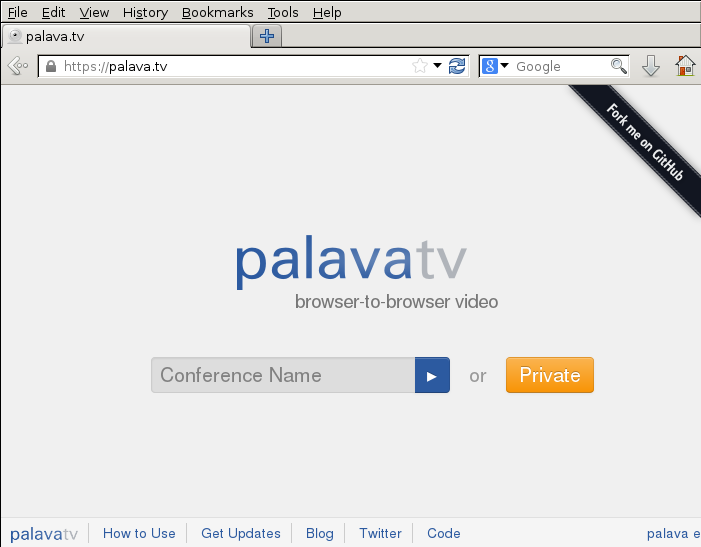
\includegraphics[height=0.7\textheight]{img/ssl_verified.png}
    \end{center}
\end{frame}

\begin{frame}
    \frametitle{SSL im Browser}
    \begin{center}
	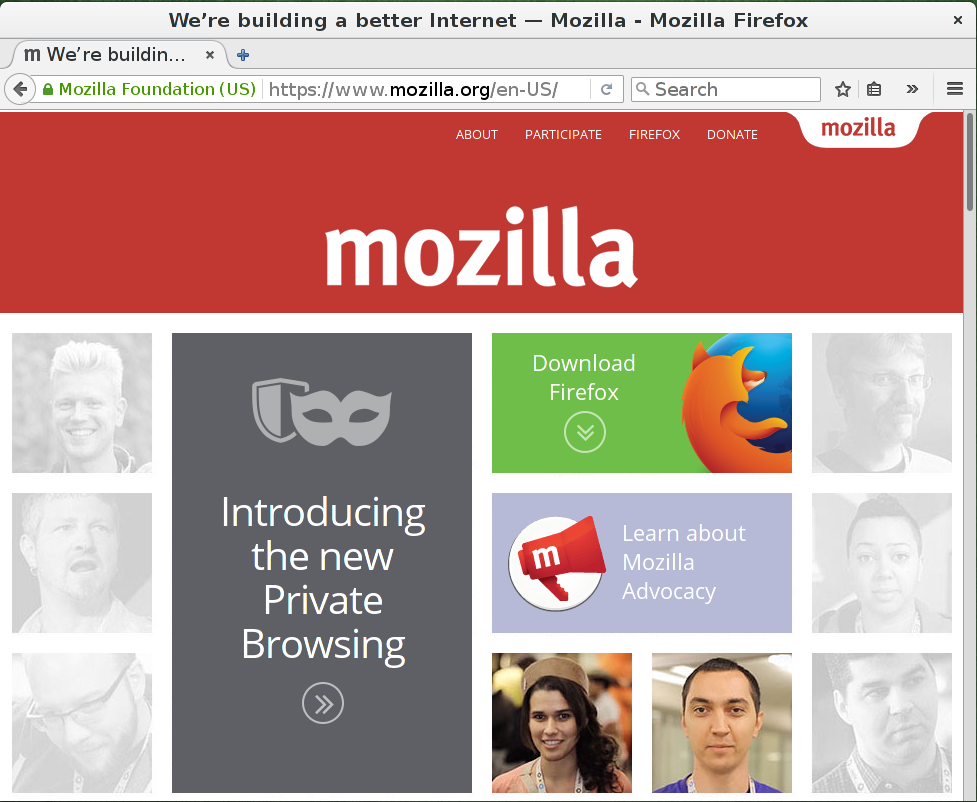
\includegraphics[height=0.7\textheight]{img/ssl_special.png}
    \end{center}
\end{frame}

\begin{frame}
    \frametitle{SSL im Browser}
    \begin{center}
	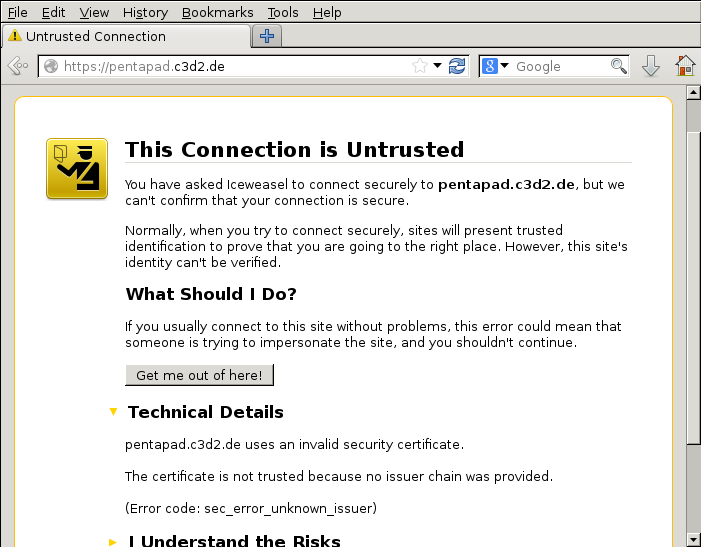
\includegraphics[height=0.7\textheight]{img/ssl_unverified.png}
    \end{center}
\end{frame}

\begin{frame}
  \frametitle{HTTPS Everywhere}
    \begin{center}
      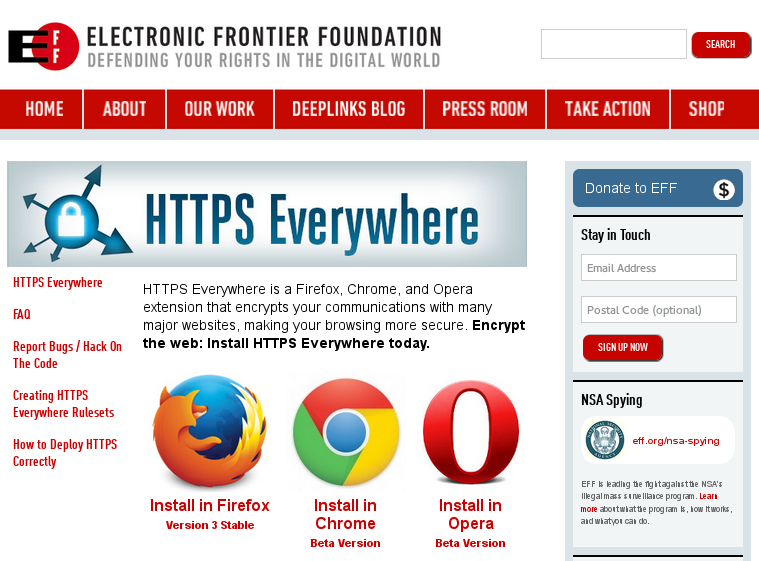
\includegraphics[height=5cm]{img/https-everywhere.png}
    \end{center}
\end{frame}
%% http://www.theconnectivist.com/2013/06/the-expanding-consolidation-of-the-consumer-internet/

\begin{frame}
    \frametitle{Lavabit}
    \begin{center}
	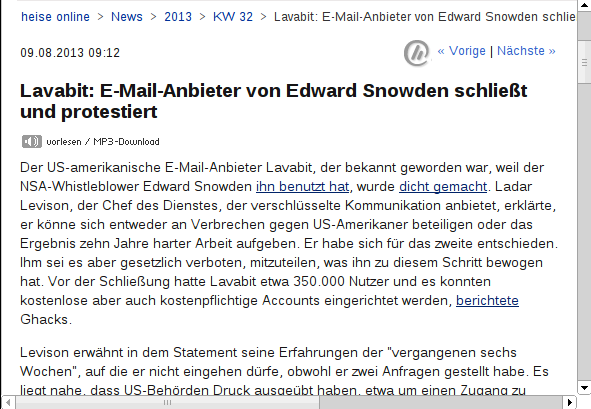
\includegraphics[height=0.6\textheight]{img/heise_lavabit.png}
    \end{center}
\end{frame}

\begin{frame}
  \frametitle{Ende-zu-Ende-Verschlüsselung I}
  \begin{center}
	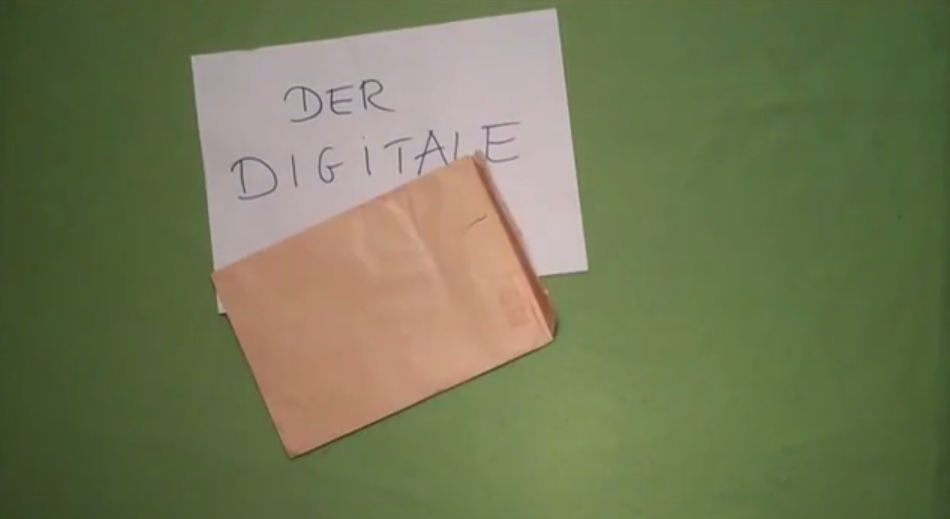
\includegraphics[height=0.6\textheight]{img/gpgvideo.png}
  \end{center}
\end{frame}

\begin{frame}
    \frametitle{Ende-zu-Ende-Verschlüsselung II}
    \begin{itemize}\Large
      \item Email: GPG = Gnu Privacy Guard
      \item Thunderbird: Enigmail
      \item Outlook: Gpg4win
      \item Apple Mail: GPGTools
      \item Web: Mailvelope (Firefox, Chrome)
    \end{itemize}
\end{frame}

\begin{frame}
  \frametitle{E-Mail-Selbstverteidigung}
  \begin{center}
    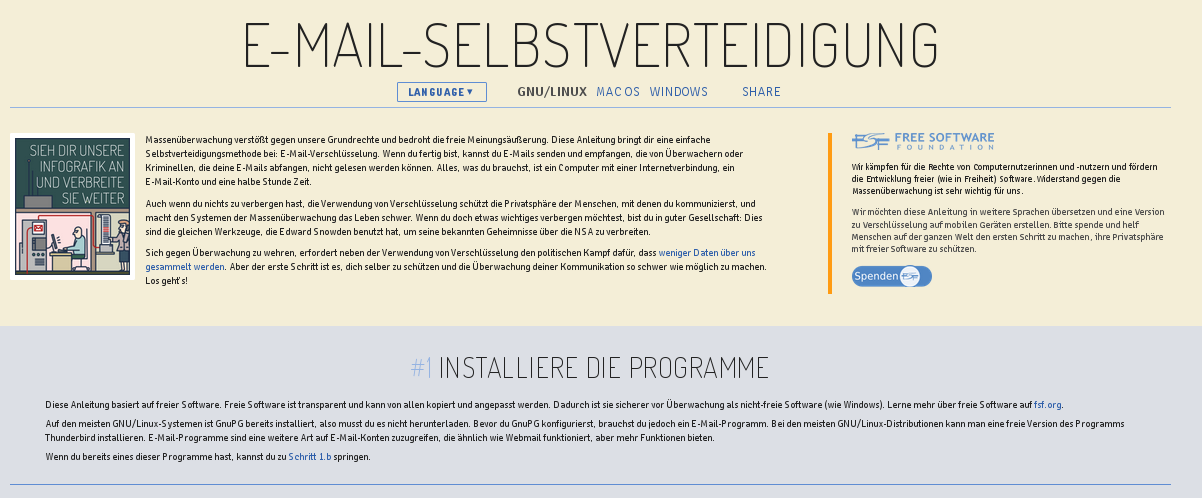
\includegraphics[height=0.5\textheight]{img/emailselfdefense.png}
    \begin{itemize}
      \item https://emailselfdefense.fsf.org/de/
    \end{itemize}	
  \end{center}	
\end{frame}

\begin{frame}
  \frametitle{Ende-zu-Ende-Verschlüsselung III}
  \begin{itemize}
    \item<2-> OTR für Jabber:
      \begin{itemize}
        \item Pidgin mit OTR-Plugin für Linux und Windows
        \item GibberBot oder Xabber für Android
        \item Adium für Mac, ChatSecure für iOS
      \end{itemize}
    \item<3-> palava.tv oder Linphone für Videotelefonie
    \item<4-> Redphone für Handytelefonate (Android)
    \item<5-> TextSecure für Nachrichten (Android)
  \end{itemize}
\end{frame}

\begin{frame}
  \frametitle{TextSecure}
    \begin{center}
      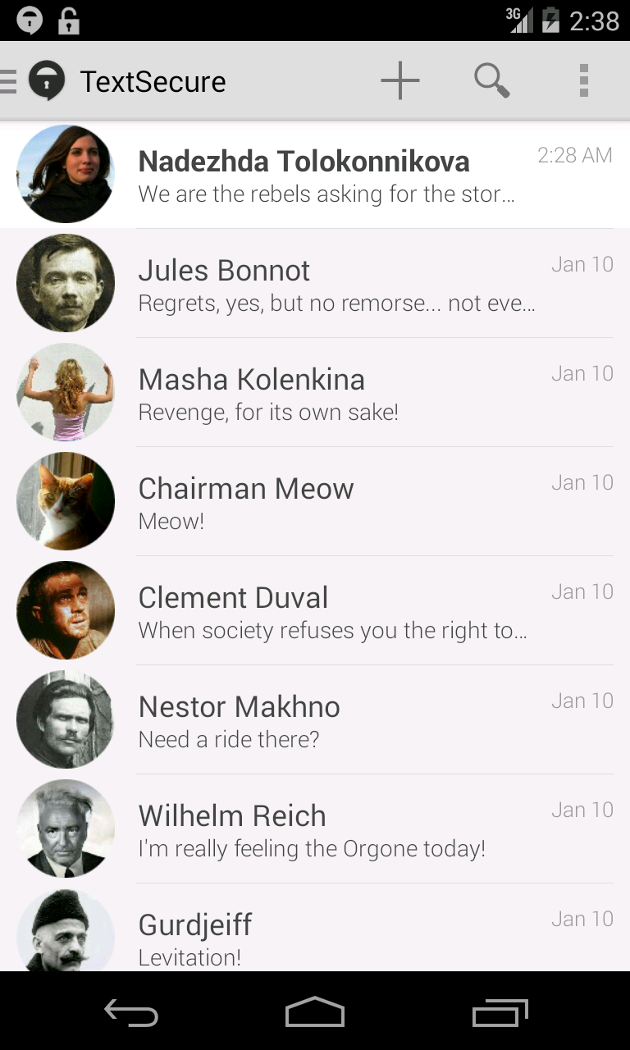
\includegraphics[height=6cm]{img/textsecure1.png}
      \hspace{0.5cm}
      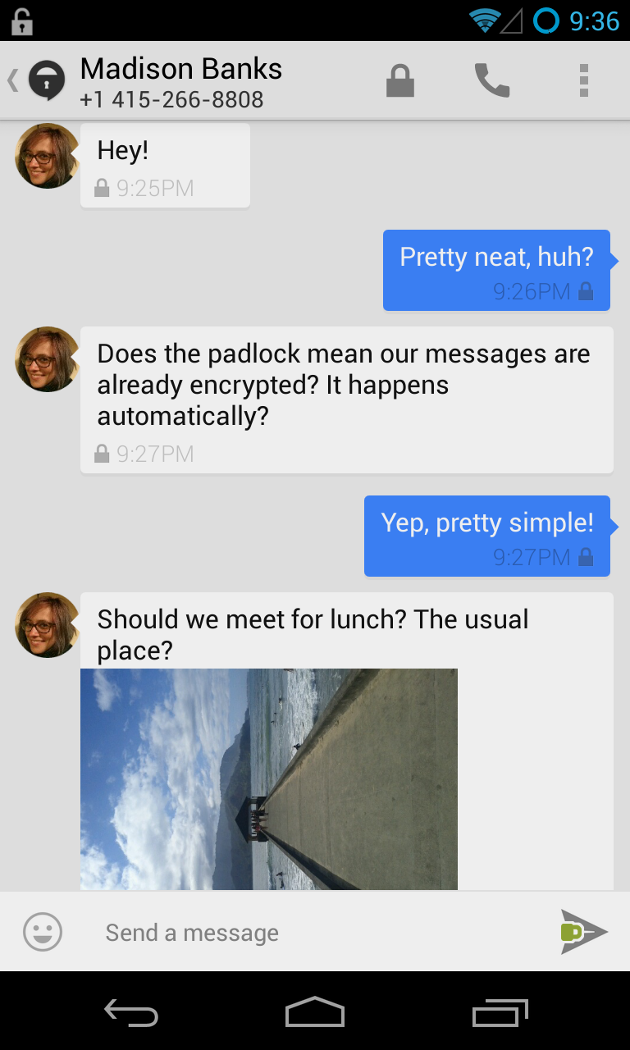
\includegraphics[height=6cm]{img/textsecure2.png}
    \end{center}
\end{frame}

\begin{frame}
    \frametitle{Metadaten - Lightbeam}
    \begin{center}
	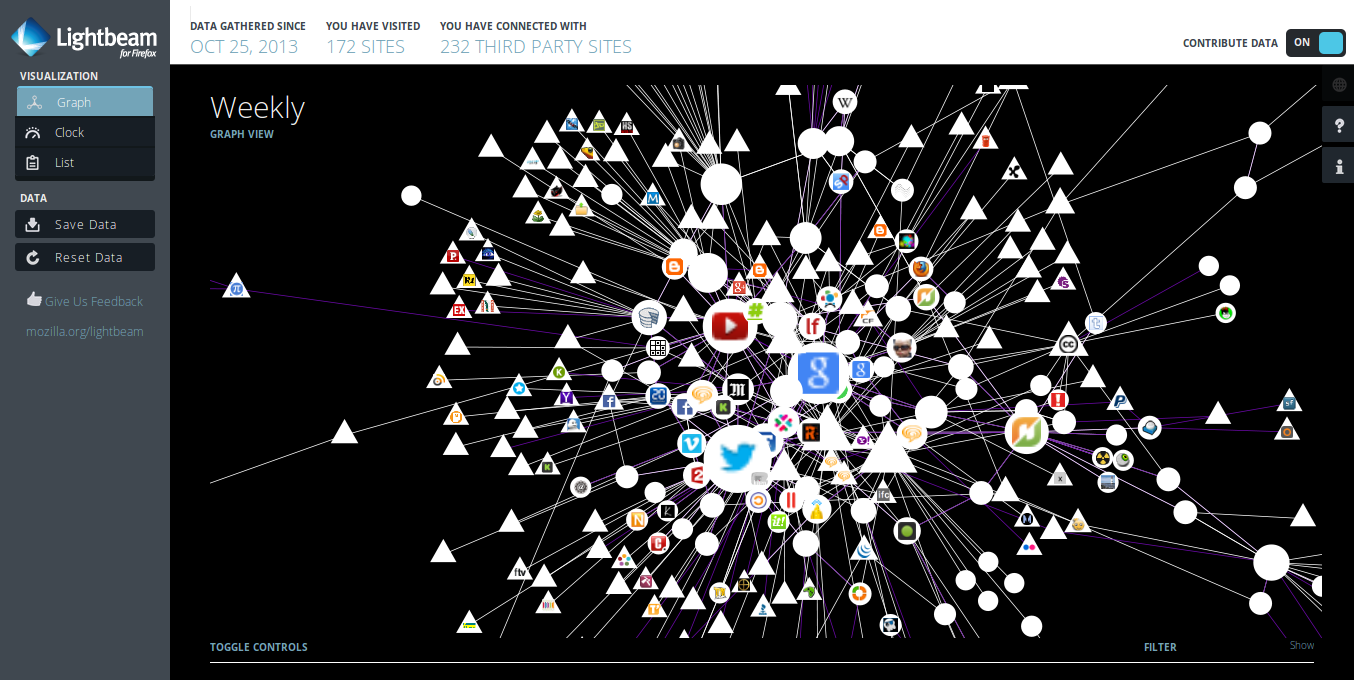
\includegraphics[height=0.7\textheight]{img/lightbeam.png}
	\\{\small \href{http://www.flickr.com/photos/8517757@N03/10538205035/in/photolist-h4e4dg}{Grafik:} \href{http://creativecommons.org/licenses/by-sa/3.0/deed.en}{\cc{by-sa}} Clint Lalonde}
    \end{center}
\end{frame}

\begin{frame}
  \frametitle{Metadaten - Disconnect}
  \begin{center}
	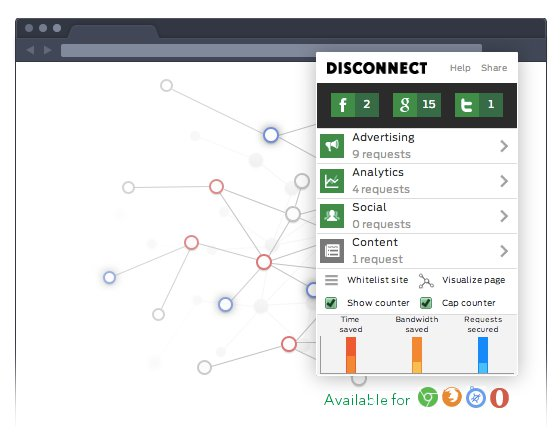
\includegraphics[height=0.7\textheight]{img/disconnectme.jpg}
  \end{center}
\end{frame}

%%\section{Metadaten}
%%\subsection{}

%%\begin{frame}
%%    \frametitle{Tor}
%%    \begin{center}
%%	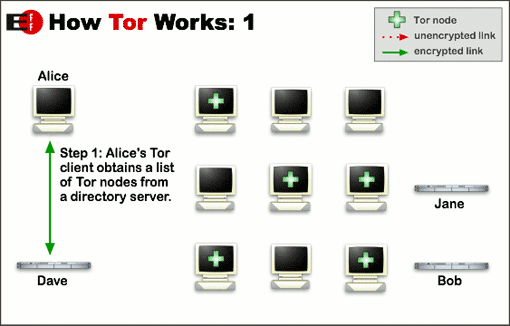
\includegraphics[height=0.7\textheight]{img/tor1.png}
%	\\{\small \href{https://www.torproject.org/images/htw1.png}{Grafik}: \href{https://creativecommons.org/licenses/by/3.0/us/}{\cc{by}} The Tor Project}
%%    \end{center}
%%\end{frame}

%%\begin{frame}
%%    \frametitle{Tor}
%%    \begin{center}
%%	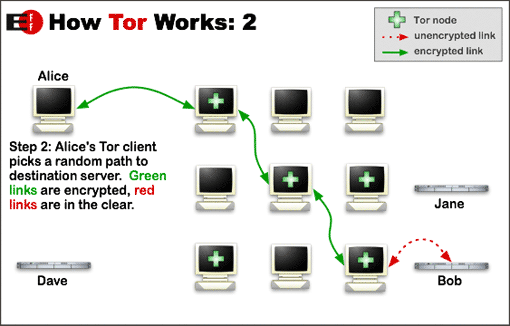
\includegraphics[height=0.7\textheight]{img/tor2.png}
%%	\\{\small \href{https://www.torproject.org/images/htw2.png}{Grafik}: \href{https://creativecommons.org/licenses/by/3.0/us/}{\cc{by}} The Tor Project}
%%    \end{center}
%%\end{frame}

%%\begin{frame}
%%    \frametitle{Tor}
%%    \begin{center}
%%	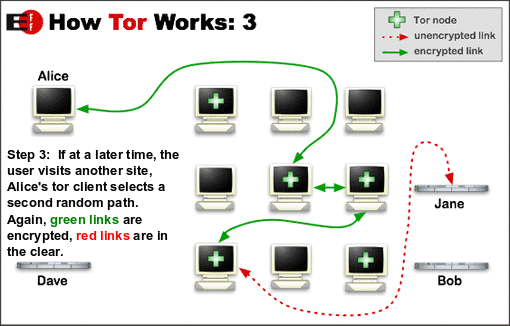
\includegraphics[height=0.7\textheight]{img/tor3.png}
%%	\\{\small \href{https://www.torproject.org/images/htw3.png}{Grafik}: \href{https://creativecommons.org/licenses/by/3.0/us/}{\cc{by}} The Tor Project}
%%    \end{center}
%%\end{frame}

%%\begin{frame}
%%  \frametitle{Tor}
%%  \begin{center}
%%	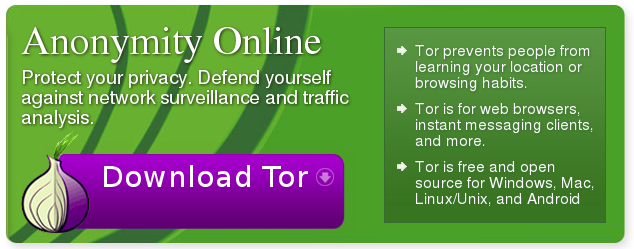
\includegraphics[height=0.5\textheight]{img/tor-banner.png}
%%  \end{center}
%%\end{frame}

%%\begin{frame}
%%    \frametitle{Anonymität unter Vollüberwachung}
%%    \begin{center}
%%	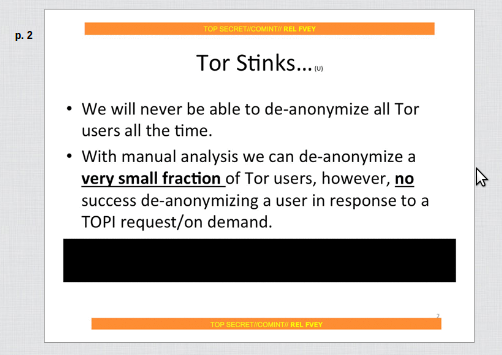
\includegraphics[height=0.7\textheight]{img/torstinks.png}
%%    \end{center}
%%\end{frame}

%%\begin{frame}
%%    \frametitle{Torroristen}
%%    \begin{center}
%%	
\includegraphics[width=0.8\textheight]{img/torrorist.png}
%%    \end{center}
%%\end{frame}

\section{Verhalten}
\subsection{}

\begin{frame}
  \frametitle{Dezentrale Dienste}
    \begin{columns}
        \begin{column}{5cm}
            \begin{center}
                
\includegraphics[height=0.2\textheight]{img/mail.pdf} \\
                E-Mail \\
                \vspace{1cm}
                
\includegraphics[height=0.2\textheight]{img/jabber.png}
            \end{center}
        \end{column}
        \begin{column}{5cm}
            \begin{center}
                
\includegraphics[height=0.2\textheight]{img/bitmessagelogo.png} \\
                Bitmessage \\
                \vspace{1cm}
                
\includegraphics[width=0.8\textwidth]{img/palava-tv.png}
            \end{center}
        \end{column}
    \end{columns}
\end{frame}

\begin{frame}
    \frametitle{Alternative Suchmaschinen}

    \begin{columns}
        \begin{column}{5cm}
            \begin{center}
                    \begin{itemize}
                            \item Startpage
                            \vspace{2cm}
                            \item DuckDuckGo
                    \end{itemize}
            \end{center}
        \end{column}
        \begin{column}{5cm}
            \begin{center}
                
\includegraphics[width=0.5\textwidth]{img/startp_logo.png}
                \vspace{1cm}
                
\includegraphics[width=0.8\textwidth]{img/duckduckgo.pdf}
            \end{center}
        \end{column}
    \end{columns}
\end{frame}

\begin{frame}
    \frametitle{Datensparsamkeit}
    \begin{itemize}
        \item<2-> Viele Daten zusammen ergeben Profile
        \item<3-> Werden die Daten gebraucht?
        \item<4-> Werden echte Daten gebraucht?
            \begin{itemize}
              \item<5-> Pseudonymität
              \item<6-> mailinator.com (Wegwerf-Email-Adresse)
              \item<7-> frank-geht-ran.de (Wegwerf-Telefonnummer)
              \item<8-> bugmenot.com (Fake Accounts)
            \end{itemize}
    \end{itemize}
\end{frame}

\begin{frame}
    \frametitle{Passwörter}
    \begin{itemize}
        \item<2-> Keine einfachen Wörter
        \item<3-> Groß-, Kleinbuchstaben, Ziffern, Sonderzeichen
        \item<4-> Beispiele:
            \begin{itemize}
                \item<5-> dragon
                \item<6-> (nCuAj.§Tsm!f
                \item<7-> IchLiebeDich
                \item<8-> .§)=/)=`
                \item<9-> qwerty
                \item<10-> Mks?o/.u,1Psw!
            \end{itemize}
        \item<12-> Verschiedene Passwörter nutzen!
        \item<13-> Passwort-Manager verwenden \\ (z.B. Keepass, Password Safe)
    \end{itemize}
\end{frame}

\begin{frame}
  \frametitle{Diskussion}
  \begin{center}
    {\Large Diskussion}\\
    \vspace{5mm}
    \href{https://github.com/c3d2/cms-nsa}{Folien}: \href{https://creativecommons.org/licenses/by-sa/4.0/}{\cc{by-sa}} Chaos Computer Club Dresden \\
    \vspace{4mm}
    CMS Dresden: schule@c3d2.de
  \end{center}
\end{frame}

\end{document}
